\title{クラウドファンディングにおける成功の判別分析}
\author{プロジェクトマネジメントコース\\
ソフトウェア開発管理グループ\\
矢吹研究室\\
1242105\\
三浦泰介}
\date{}
\begin{document}
\maketitle

\chapter*{謝辞}

\tableofcontents%目次

\chapter{序論}
\section{本章の構成}
本章では,本研究の背景・目的・方法・プロジェクトマネジメントとの関係性を記す.
\section{研究の背景}
クラウドファンディングと呼ばれるインターネットを用いた資金調達の手法が,近年,世界中ではやりを見せており,日本においてもクラウドファンディングを利用して資金調達を行う,プロジェクトが数多く出てきている.クラウドファンディングは誰でも行う権利があり,プロジェクトの規模の大きさも問わないため多くのアーティストやベンチャー企業などから注目を集めており,数多くのいままでになかった製品やサービスが実現化している.プロジェクトにおいて資金集めは極めて重要であり,当然,資金集めができなければプロジェクトは破綻してしまうため,クラウドファンディングを利用する場合は,まずはプロジェクトの成功させる前にクラウドファンディングという一つのプロジェクトを成功させなければならない.クラウドファンディングの成功の有無に関わる成功要因を明らかにし,クラウドファンディングを行う人や出資する人の参考になる情報を見つけられないか考えた.

 現在,クラウドファンディングは資金提供者に対するリターンの形で3つの種類に分類分けをされている.
\begin{description}
 \item[寄付型] 金銭的リターンのない
 \item[投資型] 金銭的リターンのある
 \item[購入型] 権利や物品を購入することで支援する
\end{description}
日本では金融商品取引法が2014 年に改正されるまで,法規制の問題から,見返りを得ない寄付型,購入型に限られていた.購入型はリターンがあるためリターンを目当てに多くの出資者が集まる傾向があり,購入型は日本で一番市場が大きいクラウドファンディングの形態である.今回は市場が,最も大きい購入型のプロジェクトの成功率に関わる成功要因を探すこととする.

\section{研究目的}
 クラウドファンディングサイトに掲載されているプロジェクトから,支援の金額,コースの数など支援者側から見える情報をデータとして集め,決定木を描くことで,クラウドファンディングにおける成功要因を明らかにし,クラウドファンディングを用いたプロジェクトを行う際や投資する際の参考となる指標を作ることを目的とする.

\section{研究方法}
監視するクラウドファンディングサイトの選定を行い,毎日定時にデータ収集を行う.プロジェクトの内容や,代表者から知り得る情報を元にデータマイニングの手法の一つである決定木分析を用いて,成功の成否に繋がるパターンを見つけ出す.また成功予測を行い,実際の成否と一致率を上げることで憑性を確保する.

\section{プロジェクトマネジメントとの関連性}
クラウドファンディングを成功させるまでを一つのプロジェクトと考え,その成功率をあげることクラウドファンディングで資金調達を行うプロジェクトの成功率をあげることに繋がると考える.


\chapter{クラウドファンディングについて}
\section{本章の構成}
本章では,研究対象であるクラウドファンディングについて解説を記す.

\section{クラウドファンディングとは}
クラウドファンディングとは活動資金が必要な組織や団体に不特定多数の人がインターネットを経由し,資金提供を行うことを指す.群衆(crowd)資金調達(funding)を組み合わせた造語であり,ソーシャルファンディングと呼ばれることもある.

\section{クラウドファンディングの種類}
クラウドファンディングは資金提供者に対するリターンの形で3つの種類に分類分けがされている.
\begin{description}
 \item[寄付型] 金銭的リターンのない
 \item[投資型] 金銭的リターンのある
 \item[購入型] 権利や物品を購入することで支援する
\end{description}
日本においては購入型が最も認知されており,プロジェクト数も多い.

\section{クラウドファンディングの歴史}
クラウドファンディングの雛形の前身は17世紀に活躍した書籍編集者のジョン・テイラー氏が,書籍の印刷代を募るために使われた寄付ビジネスモデルだったと言われている.寄付のリターンが標題紙に名前を掲載する権利を提供することであり,現在でも映画のスタッフロールや出版物に名前が掲載されることはポピュラーなリターンとして行われており,クラウドファンディングと通じるものがあるとされている.

\chapter{目的}

\chapter{手法}

\chapter{結果}

\chapter{考察}

\chapter{結論}

%図の挿入
\begin{figure}[htb]
\centering
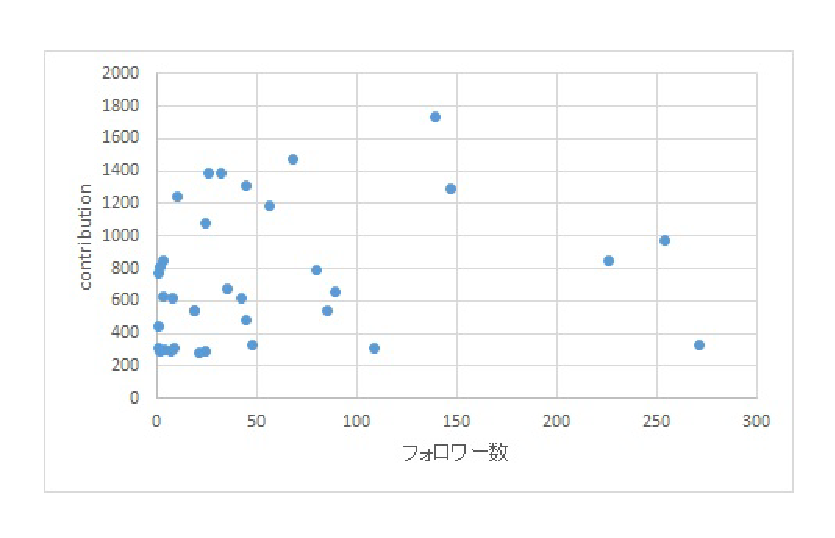
\includegraphics[width=10cm]{figure.pdf}
\caption{図の挿入例}\label{サンプル図}
\end{figure}

参考文献は文献ファイル(この文書では\verb|biblio.bib|)に記述し,\verb|\cite|で参照する.例:データベースのための問い合わせ言語SQLで数独を解く方法が提案されている\cite{yabuki2011}.このように参照すると,参考文献リストに自動的に登録される.文献の種類には,雑誌論文\cite{yabuki2011}や会議録論文\cite{yabuki2013},卒業論文\cite{kubo2014},書籍\cite{okumura2013},ウェブサイト\cite{self}などがある.文献の種類によって必要な項目が異なるため,\verb|biblio.bib|を見て確認すること.

\bibliographystyle{junsrt}
\bibliography{biblio}%「biblio.bib」というファイルが必要.

\end{document}
